\setcounter{section}{0}

\Needspace{5\baselineskip}
\hypertarget{generative-adversarial-networks-gans}{%
\section{Generative Adversarial Networks (GANs)}\label{generative-adversarial-networks-gans}}

\Needspace{5\baselineskip}
\hypertarget{i.-core-idea-2}{%
\subsection{I. Core Idea}\label{i.-core-idea-2}}

\Needspace{5\baselineskip}
Generative adversarial networks are an ingenious and powerful unsupervised learning framework proposed by Ian Goodfellow in 2014. Their core idea is to establish a ``two-player game.'' Imagine two competing neural networks:

Generator (G): its job is to create realistic-looking data ``out of thin air'' (for example, counterfeit Picasso paintings). It tries to imitate the distribution of real data.

Discriminator (D): its job is to act as an ``authentication expert,'' judging whether input data come from the real dataset (genuine Picasso paintings) or are forged by the generator (counterfeit paintings).

They evolve together through ``adversarial'' interaction: generator G learns diligently, trying to produce increasingly realistic data to ``deceive'' discriminator D; discriminator D learns diligently, trying to improve its judgment and accurately ``see through'' every forgery from G. This resembles an arms race. The eventual ideal state is that G becomes so capable that its ``fakes'' pass for real. As will be proved later, D can then no longer distinguish them and can only guess (assigning a 50\% probability of being real).

\Needspace{5\baselineskip}
\hypertarget{ii.-objective-function}{%
\subsection{II. Objective Function}\label{ii.-objective-function}}

\[
\min_G \max_D V(D, G)=\mathbb{E}_{x\sim p_{data}(x)}[\log D(x)] + \mathbb{E}_{z\sim p_z(z)}[\log(1 - D(G(z)))]
\]

\Needspace{4\baselineskip}
\begin{enumerate}
\def\labelenumi{\arabic{enumi}.}
\tightlist
\item
  Notation and players
\end{enumerate}

\begin{itemize}
\tightlist
\item
  \(G\) (generator): our ``forger,'' a neural network.
\item
  \(D\) (discriminator): our ``authentication expert,'' also a neural network.
\item
  \(x\): a real datum (such as a genuine photograph of a cat).
\item
  \(p_{data}(x)\): the probability distribution of real data (theoretically, the collection of all genuine cat photographs). \(x \sim p_{data}(x)\) means that \(x\) is a sample drawn randomly from this real dataset.
\item
  \(z\): a random noise vector (usually sampled from a simple distribution, such as a Gaussian or uniform distribution). \(z\) is the source of \(G\)'s creative ``inspiration.''
\item
  \(p_z(z)\): the distribution of noise vector \(z\). \(z \sim p_z(z)\) means that \(z\) is a sample drawn randomly from this noise distribution.
\end{itemize}

\Needspace{4\baselineskip}
\begin{enumerate}
\def\labelenumi{\arabic{enumi}.}
\setcounter{enumi}{1}
\tightlist
\item
  Network inputs and outputs
\end{enumerate}

\begin{itemize}
\tightlist
\item
\Needspace{5\baselineskip}
  \(G(z)\):

  \begin{itemize}
  \tightlist
  \item
    Input: noise \(z\).
  \item
    Output: a ``forged'' datum. \(G\) tries to make \(G(z)\) look as real as \(x\).
  \end{itemize}
\item
\Needspace{5\baselineskip}
  \(D(x)\):

  \begin{itemize}
  \tightlist
  \item
    Input: a datum (either real \(x\) or forged \(G(z)\)).
  \item
    Output: a probability between 0 and 1, expressing the probability that \(D\) believes the input is real.
  \item
    \(D(x)\to 1\) means that \(D\) considers \(x\) very likely to be real.
  \item
    \(D(x)\to 0\) means that \(D\) considers \(x\) very likely to be forged.
    It should be clarified that, for data \(x\), the true value of \(D(x)\) follows a 0--1 distribution, but the probability distribution of \(x\) is not a 0--1 distribution. When cross-entropy loss is used here, the corresponding probability distribution in the function should be the distribution of \(D(x)\), not \(p_{data}(x)\), the distribution of \(x\).
  \end{itemize}
\end{itemize}

\(p_{data}(x)\) is the probability density distribution of \(x\) itself. It need not take the discrete form \(p(x=\cdots)=\cdots\); more likely, it is a theoretical, implicit, unknown probability density distribution, the ``target distribution'' that our model tries to learn and simulate. For example, imagine an ideal, perfect function \(p_{data}\) in the universe that is the probability density function of all images. Given a realistic, natural face image, it outputs a high probability density of \(0.0001\); given an unusual image, it outputs a lower probability value of \(10^{-20}\). Theoretically, \(p_{data}(x)\) contains the generative patterns of all ``valid'' data within the scope of study (such as all faces).

Although we do not have the probability density function \(p_{data}\) itself, we have results sampled from it. These ``sampled results'' are your ``training dataset''; for example, ImageNet is a set of samples from \(p_{data}(x)\), where \(x\) represents ``natural images.'' In the GAN objective, the practical meaning of \(\mathbb{E}_{x\sim p_{data}(x)}\) is ``randomly draw a batch of data \(x\) from your training dataset.'' We use this empirical distribution to approximate \(p_{data}\). As GAN training proceeds, ``realistic'' means that the distribution of the data (images) generated by \(G\) approaches the distribution in the given dataset. In fact, we consider this an end-to-end approximation of the extremely complex function \(p_{data}\). We need generative models such as GANs precisely because \(p_{data}(x)\) is too complex to model directly using traditional methods (such as maximum likelihood estimation), so we can only learn it indirectly through this ``game.''

\Needspace{4\baselineskip}
\begin{enumerate}
\def\labelenumi{\arabic{enumi}.}
\setcounter{enumi}{2}
\tightlist
\item
  Term-by-term explanation of the objective
\end{enumerate}

\Needspace{5\baselineskip}
Now consider its two main parts:

\[
V(D,G)=\mathbb{E}_{x\sim p_{data}(x)}[\log D(x)] + \mathbb{E}_{z\sim p_z(z)}[\log(1-D(G(z)))]
\]

\begin{itemize}
\tightlist
\item
  First term: \(\mathbb{E}_{x\sim p_{data}(x)}[\log D(x)]\)

  \begin{itemize}
  \tightlist
  \item
    Meaning: measures how well discriminator \(D\) correctly identifies real data.
  \item
    \(D\)'s objective (\(\max_D\)): \(D\) wants to maximize this term.

    \begin{itemize}
    \tightlist
    \item
      Given real data \(x\), \(D\) wants its output \(D(x)\) as close to 1 as possible (``I am certain this is real'').
    \item
      As \(D(x)\to 1\), \(\log D(x)\) approaches \(\log(1)=0\), the maximum of the \(\log\) function over its domain here (0 to 1).
    \end{itemize}
  \item
    \(G\)'s objective: \(G\) cannot control this term because it depends only on real data \(x\).
  \end{itemize}
\item
  Second term: \(\mathbb{E}_{z\sim p_z(z)}[\log(1-D(G(z)))]\)

  \begin{itemize}
  \tightlist
  \item
    Meaning: measures how well discriminator \(D\) correctly identifies forged data.
  \item
    \(D(G(z))\): \(D\)'s judgment of fake data \(G(z)\) produced by \(G\) (its estimated probability that \(G(z)\) is real).
  \item
    \(1-D(G(z))\): the probability that \(D\) considers \(G(z)\) forged.
  \item
    \(D\)'s objective (\(\max_D\)): \(D\) wants to maximize this term.

    \begin{itemize}
    \tightlist
    \item
      Given forged data \(G(z)\), \(D\) wants its output \(D(G(z))\) as close to 0 as possible (``I am certain this is fake'').
    \item
      As \(D(G(z))\to 0\), \(1-D(G(z))\) approaches 1, so \(\log(1-D(G(z)))\) approaches \(\log(1)=0\).
    \item
      Thus, by making both \(\log D(x)\) and \(\log(1-D(G(z)))\) approach 0, \(D\) maximizes \(V(D,G)\).
    \end{itemize}
  \item
    \(G\)'s objective (\(\min_G\)): \(G\) wants to minimize this term (because \(G\) cannot affect the first term).

    \begin{itemize}
    \tightlist
    \item
      \(G\) aims to ``deceive'' \(D\). It wants \(D\) to mistake \(G(z)\) for real data, making \(D(G(z))\) as close to 1 as possible.
    \item
      As \(D(G(z))\to 1\), \(1-D(G(z))\) approaches 0.
    \item
      \(\log(1-D(G(z)))\) approaches \(\log(0)=-\infty\).
    \item
      In this way, \(G\) successfully minimizes \(V(D,G)\).
    \end{itemize}
  \end{itemize}
\end{itemize}

\Needspace{4\baselineskip}
\begin{enumerate}
\def\labelenumi{\arabic{enumi}.}
\setcounter{enumi}{3}
\tightlist
\item
  Summary: \(\min_G \max_D V(D,G)\)
\end{enumerate}

\begin{itemize}
\tightlist
\item
\Needspace{5\baselineskip}
  \(\max_D V(D,G)\) (the discriminator's objective): \(D\) tries to maximize \(V(D,G)\), learning to:

  \begin{enumerate}
  \def\labelenumi{\arabic{enumi}.}
  \tightlist
  \item
    Output \(D(x)=1\) for real data \(x\).
  \item
    Output \(D(G(z))=0\) for forged data \(G(z)\). If \(D\) is a perfect discriminator, the maximum of \(V(D,G)\) is \(0+0=0\).
  \end{enumerate}
\item
\Needspace{5\baselineskip}
  \(\min_G V(D,G)\) (the generator's objective): \(G\) tries to minimize \(V(D,G)\), learning to:

  \begin{enumerate}
  \def\labelenumi{\arabic{enumi}.}
  \tightlist
  \item
    Generate \(G(z)\) that misleads \(D\), making \(D(G(z))=1\). As \(G\) becomes stronger, the second term \(\log(1-D(G(z)))\) is pushed toward \(-\infty\).
  \end{enumerate}
\end{itemize}

\Needspace{4\baselineskip}
\begin{enumerate}
\def\labelenumi{\arabic{enumi}.}
\setcounter{enumi}{4}
\tightlist
\item
  Further discussion of the objective
\end{enumerate}

\Needspace{4\baselineskip}
\begin{enumerate}
\def\labelenumi{(\arabic{enumi})}
\tightlist
\item
  Discriminator D's objective
\end{enumerate}

Notice that \(V(D, G)\) closely resembles binary cross-entropy loss. Treat \(D\) as a binary classifier: real data \((x)\) have label \(y=1\), and forged data \((G(z))\) have label \(y=0\). \(D\) aims to minimize classification cross-entropy, equivalently maximizing \(V(D, G)\) above.

\Needspace{4\baselineskip}
\begin{enumerate}
\def\labelenumi{\arabic{enumi}.}
\tightlist
\item
  Standard binary cross-entropy (BCE) loss
\end{enumerate}

First, recall the standard binary cross-entropy loss, typically used for binary classification (such as deciding ``yes'' or ``no'').

\Needspace{5\baselineskip}
Suppose:

\begin{itemize}
\tightlist
\item
  \(y\) is the true label (\(y=1\) means ``real'' and \(y=0\) means ``fake'').
\item
  \(p\) is the model's predicted probability that \(y=1\).
\end{itemize}

\Needspace{5\baselineskip}
Then the BCE loss \(L\) for a single sample is:

\[
L(y,p) = -[y\cdot\log(p) + (1-y)\cdot\log(1-p)]
\]

\Needspace{5\baselineskip}
This formula means:

\begin{itemize}
\tightlist
\item
  If \(y=1\) (the true label is ``real''), the loss becomes \(L=-[1\cdot\log(p)+0]=-\log(p)\).

  \begin{itemize}
  \tightlist
  \item
    To minimize \(L\), maximize \(\log(p)\), making \(p\to 1\).
  \end{itemize}
\item
  If \(y=0\) (the true label is ``fake''), the loss becomes \(L=-[0+1\cdot\log(1-p)]=-\log(1-p)\).

  \begin{itemize}
  \tightlist
  \item
    To minimize \(L\), maximize \(\log(1-p)\), making \(p\to 0\).
  \end{itemize}
\end{itemize}

This exactly matches what we expect from a classifier.

Now treat discriminator \(D\) as a binary classifier whose task is to label input data ``real'' or ``fake.''

\begin{itemize}
\tightlist
\item
  \textbf{Input 1: real data \(x\)}

  \begin{itemize}
  \tightlist
  \item
    \(D\)'s objective: classify them as ``real.''
  \item
    True label: \(y=1\).
  \item
    \(D\)'s prediction: \(p=D(x)\).
  \item
    By the BCE formula, the corresponding loss is \(L_{real}=-\log(D(x))\).
  \end{itemize}
\item
  \textbf{Input 2: forged data \(G(z)\)}

  \begin{itemize}
  \tightlist
  \item
    \(D\)'s objective: classify them as ``fake.''
  \item
    True label: \(y=0\).
  \item
    \(D\)'s prediction: \(p=D(G(z))\).
  \item
    By the BCE formula, the corresponding loss is \(L_{fake}=-\log(1-D(G(z)))\).
  \end{itemize}
\end{itemize}

\Needspace{5\baselineskip}
The discriminator's total loss is therefore:

\[
L_D = L_{real} + L_{fake} = \mathbb{E}[-\log D(x)] + \mathbb{E}[-\log(1-D(G(z)))]
\]

\[
L_D = -\Bigl(\mathbb{E}[\log D(x)] + \mathbb{E}[\log(1-D(G(z)))]\Bigr)
\]

(For brevity, we temporarily omit \(x\sim p_{data}\) and \(z\sim p_z\) outside the expectation symbol \(\mathbb{E}\).)

\Needspace{5\baselineskip}
Now return to the GAN objective \(V(D,G)\):

\[
V(D,G)=\mathbb{E}[\log D(x)] + \mathbb{E}[\log(1-D(G(z)))]
\]

\Needspace{5\baselineskip}
Comparing \(L_D\) and \(V(D,G)\) clearly shows:

\[
V(D,G) = -L_D
\]

\Needspace{4\baselineskip}
\begin{enumerate}
\def\labelenumi{(\arabic{enumi})}
\setcounter{enumi}{1}
\tightlist
\item
  Generator G's objective
\end{enumerate}

Under the original formula, generator \(G\) minimizes \(\mathbb{E}[\log(1-D(G(z)))]\). This objective is theoretically perfect, but in practice, particularly early in training, it causes a serious problem: vanishing gradients.

\Needspace{5\baselineskip}
Let us examine why:

\begin{enumerate}
\def\labelenumi{\arabic{enumi}.}
\tightlist
\item
  Early in training, \(G\) is poor: initially, \(G\) is simply a random neural network, and its outputs \(G(z)\) are meaningless noise (such as television static).
\item
  \(D\) can easily ``overwhelm'' \(G\): discriminator \(D\) has a simple task, distinguishing ``real cats'' from ``television static.'' \(D\) learns quickly and confidently identifies \(G\)'s outputs \(G(z)\) as fake.
\item
  What happens to \(D\)'s output?

  \begin{itemize}
  \tightlist
  \item
    When \(D\) sees \(G(z)\) (static), it is certain the input is fake.
  \item
    Consequently, \(D(G(z))\) is very close to 0.
  \end{itemize}
\item
  What goes wrong with \(G\)'s loss?

  \begin{itemize}
  \tightlist
  \item
    \(G\)'s loss is \(L_G=\log(1-D(G(z)))\).
  \item
    If \(D(G(z))\) is near 0 (say 0.001), then \(L_G\) is \(\log(1-0.001)\approx \log(1)=0\).
  \item
    \(G\)'s loss appears ``low'' (near 0), but this is misleading. The real problem is the gradient.
  \end{itemize}
\end{enumerate}

\Needspace{5\baselineskip}
Consider the graph of \(G\)'s loss \(L_G=\log(1-p)\), where \(p=D(G(z))\) is \(D\)'s output:

\begin{itemize}
\tightlist
\item
  X-axis: \(D\)'s output \(p\) (from 0 to 1)
\item
  Y-axis: \(G\)'s loss \(L_G\)
\end{itemize}

\Needspace{5\baselineskip}
Observe:

\begin{itemize}
\tightlist
\item
  When \(p\) is near 0 (when \(D\) confidently judges \(G(z)\) fake), this curve is very flat.
\item
  In calculus, ``flat'' means that the slope (gradient) is near 0.
\end{itemize}

This is where disaster occurs: \(G\) produces poor images \(\rightarrow\) \(D\) confidently labels them fake (\(p\approx 0\)) \(\rightarrow\) the loss gradient received by \(G\) is \(\approx 0\) \(\rightarrow\) \(G\) cannot update its parameters and learns nothing.

This is called ``saturation'': \(G\) learns slowest precisely when it most needs to learn (when it performs worst).

The original paper's authors proposed a simple, practical correction.

They suggested that \(G\) should maximize \(\log(D(G(z)))\) rather than letting \(G\) minimize \(\log(1-D(G(z)))\).

\begin{itemize}
\tightlist
\item
  Old loss (blue): \(\log(1-p)\). As \(p \rightarrow 0\), the gradient is flat (vanishing).
\item
  New loss (green): \(-\log(p)\). As \(p \rightarrow 0\), the gradient becomes extremely steep (approaching \(-\infty\)).
\end{itemize}

This new loss has exactly the desired property: it provides a large, strong gradient signal precisely when \(G\) performs worst (when \(D(G(z))\) is near 0), allowing \(G\) to learn quickly from the start of training.

However, this still does not completely solve the vanishing-gradient problem.

\[
\nabla_{\theta_g} L_G = \nabla_{\theta_g}[-\log(D(G(z)))]
\]

\Needspace{5\baselineskip}
Using the chain rule, we split it into three parts:

\[
\nabla_{\theta_g} L_G =
\frac{d(-\log p)}{dp}
\cdot
\nabla_a D(a)\rvert_{a=G(z)}
\cdot
\nabla_{\theta_g} G(z)
\]

Here \(p=D(G(z))\) is \(D\)'s final output and \(a=G(z)\) is \(D\)'s input. The three parts correspond to the gradient from \(G\)'s loss, the gradient inside \(D\), and the gradient inside \(G\).

Part 1: the part of interest

\[
\frac{d(-\log p)}{dp}=-\frac{1}{p}
\]

\begin{itemize}
\tightlist
\item
  When \(G\) is poor, \(p=D(G(z)) \rightarrow 0\).
\item
  This term \(-\frac{1}{p}\) tends to infinity.
\item
  In other words, \(G\)'s loss itself is ``desperately'' producing an enormous signal.
\end{itemize}

Part 2: the part that ``really vanishes''

\[
\nabla_a D(a)
\]

This is \(\nabla_{G(z)}D(G(z))\), the gradient of \(D\)'s output probability \(p\) with respect to \(D\)'s input \(a\). How does \(D\) produce a probability between 0 and 1? Its final layer is a sigmoid function. \(D\) aims to separate real and fake data; when it becomes strong (with no overlap), it assigns \(G(z)\) an extremely low score. To output \(p \rightarrow 0\), the sigmoid input (logits) must be a large negative number (such as -10 or -20).

\begin{figure}[htbp]
\centering
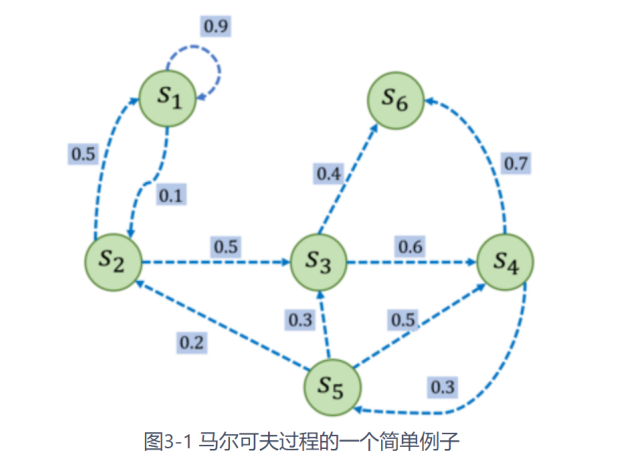
\includegraphics{images/image-0012.png}
\caption{Logistic Function}
\end{figure}

When \(x\) is very small or very large, the derivative (gradient) of the sigmoid function that converts outputs into probabilities approaches \(0\).

\Needspace{5\baselineskip}
\(G\)'s total gradient is:

\[
\nabla_{\theta_g} L_G =
(\text{tends to infinity}) \cdot (\text{tends to }0) \cdot (\text{gradient from }G)
\]

The first term comes from \(\log\), and the second from sigmoid.
In this indeterminate form, sigmoid often dominates, causing gradients to vanish. The analogy is opening a ``fire hydrant,'' only to find the ``pipe'' (the D network) blocked by ``limescale'' (the sigmoid function). When D becomes very strong, its internal sigmoid saturates (becomes flat). This ``flat'' sigmoid layer resembles an extremely narrow bottleneck clogged with limescale (its gradient approaches 0). WGAN solves this by modifying D (see below).

\Needspace{5\baselineskip}
\hypertarget{training-endpoint}{%
\subsubsection{(4) Training Endpoint}\label{training-endpoint}}

Suppose generator \(G\) is fixed, and we seek the optimal discriminator \(D^*\) that maximizes \(V(D,G)\).

\Needspace{5\baselineskip}
Our objective is:

\[
V(D,G)=\int_x p_{data}(x)\log(D(x))dx+\int_z p_z(z)\log(1-D(G(z)))dz
\]

\Needspace{5\baselineskip}
For simplicity, we know that \(G(z)\) induces a distribution of forged data \(p_g(x)\), so the second term can also be written as an integral over \(x\):

\[
V(D,G)=\int_x [p_{data}(x)\log(D(x))+p_g(x)\log(1-D(x))]dx
\]

To find \(D(x)\) that maximizes this integral, we need only examine the function inside it (the integrand) and maximize it for each \(x\).

\Needspace{5\baselineskip}
Let \(a=p_{data}(x)\) and \(b=p_g(x)\). We seek \(D\) maximizing \(f(D)=a\log(D)+b\log(1-D)\). This is a standard extremum problem: differentiate with respect to \(D\) and set the derivative to 0:

\[
\frac{df}{dD}=\frac{a}{D}-\frac{b}{1-D}=0
\]

\Needspace{5\baselineskip}
Thus:

\[
a=(a+b)D \Rightarrow D=\frac{a}{a+b}
\]

\Needspace{5\baselineskip}
Substituting back for \(a\) and \(b\) gives the optimal discriminator \(D^*(x)\):

\[
D^*(x)=\frac{p_{data}(x)}{p_{data}(x)+p_g(x)}
\]

By differentiating with respect to D, the derivation finds the D that maximizes V(D,G), namely the optimal discriminator. The formula says that a perfect discriminator's output probability D(x) should equal ``the probability that this x comes from real data'' divided by ``the total probability that it comes from real or forged data.''

Of course, training the discriminator is only a means; the final endpoint depends on the generator's output. Intuitively, if \(G\) becomes perfect and its forged data completely learn the real distribution, then \(p_g(x)=p_{data}(x)\) and \(D^*(x)=1/2\). We now rigorously prove that when \(D\) equals \(D^*\), minimizing \(\max_D V(D,G)=V(D^*,G)\) over \(G\) is equivalent to achieving this case.

\[
C(G)=\max_D V(D,G)=V(D^*,G)
\]

\[
C(G)=\mathbb{E}_{x\sim p_{data}}\left[\log\frac{p_{data}}{p_{data}+p_g}\right]
+\mathbb{E}_{x\sim p_g}\left[\log\frac{p_g}{p_{data}+p_g}\right]
\]

Note: \(p_{data}(x)\) and \(p_g(x)\) are abbreviated to \(p_{data}\) and \(p_g\) here.

\Needspace{5\baselineskip}
After some algebra, this expression can be rewritten as:

\[
C(G)=2\cdot D_{JSD}(p_{data}\parallel p_g)-2\log 2
\]

\begin{itemize}
\tightlist
\item
  \(D_{JSD}\) denotes Jensen--Shannon divergence (JSD).
\item
  Divergence is a mathematical tool in information theory for measuring differences between two probability distributions.
\end{itemize}

\Needspace{5\baselineskip}
\(G\)'s final objective is \(\min_G C(G)\), namely:

\[
\min_G [2\cdot D_{JSD}(p_{data}\parallel p_g)-2\log 2]
\]

The final mathematical objective of training generator \(G\) is to minimize the JSD between the real distribution \(p_{data}(x)\) and the forged distribution \(p_g(x)\). JSD equals \(0\) if and only if the two distributions are identical, \(p_g(x)=p_{data}(x)\). In short, the ingenious game between \(\min_G\) and \(\max_D\) in the objective turns \(G\)'s task into learning a perfect distribution \(p_g\) that matches \(p_{data}\).

\Needspace{5\baselineskip}
\hypertarget{iii.-applications-of-gans}{%
\subsection{III. Applications of GANs}\label{iii.-applications-of-gans}}

\Needspace{4\baselineskip}
\begin{enumerate}
\def\labelenumi{\arabic{enumi}.}
\tightlist
\item
  Image generation and artistic creation
\end{enumerate}

This is the best-known GAN application. The aim is to learn the ``essence'' of a large dataset (such as 100,000 face photographs), then start from a random noise vector \(z\) to generate a completely new face that is not any image in the dataset but looks extremely realistic. Models such as StyleGAN and BigGAN can generate photographs of nonexistent ``models,'' create digital art, and design game characters.

\Needspace{5\baselineskip}
Comparison with variational autoencoders (VAEs):

\textbf{GANs}

\begin{itemize}
\tightlist
\item
  Core idea: adversarial interaction, with a generator and discriminator competing.
\item
  Training objective: deceive the discriminator; \(G\) aims to make \(D\) unable to distinguish real from fake.
\item
  Generation quality: high fidelity and sharpness. Because \(D\) exists, \(G\) must generate clear, sharp edges and textures or be easily identified as fake.
\item
  Latent space \(z\): typically more entangled. The original GAN latent space \(z\) is relatively disordered; changing one dimension of \(z\) may simultaneously alter several facial features, such as hair, age, and orientation.
\end{itemize}

\textbf{VAEs}

\begin{itemize}
\tightlist
\item
  Core idea: encoding and decoding. The encoder compresses an image into a probability distribution in latent space \(z\), and the decoder samples from \(z\) and reconstructs the image.
\item
  Training objective: minimize reconstruction loss, making the decoded image as close as possible to the original.
\item
  Generation quality: relatively blurry. VAEs minimize average pixel-level error (such as \(L_2\) loss), encouraging the model to generate a ``safer'' average image.
\item
  Latent space \(z\): smoother. VAE latent space \(z\) is regularized into a continuous, smooth structure, suitable for interpolation between the \(z\) vectors of two faces.
\end{itemize}

VAEs excel at learning a smooth, meaningful latent space (useful for interpolation and understanding data structure) but generate blurrier results. GANs excel at generating highly realistic images (useful when visual fidelity is the priority) but train less stably, and their latent space is less orderly than that of VAEs.

\Needspace{4\baselineskip}
\begin{enumerate}
\def\labelenumi{\arabic{enumi}.}
\setcounter{enumi}{1}
\tightlist
\item
  Image-to-image translation
\end{enumerate}

These applications aim to transform an input image A into an output image B with a particular style or characteristic. Both input and output are images, often with some structural correspondence. Typical models include Pix2Pix (requiring paired training data, such as a sketch paired with a photograph) and CycleGAN (not requiring paired data, using cycle-consistency loss for unpaired translation). Applications include converting aerial maps to Google Maps style, colorizing black-and-white photographs, turning hand-drawn sketches into realistic photographs, converting daytime scenes to nighttime scenes, and reconstructing realistic images from semantic segmentation maps. Traditional neural network architectures in this field primarily rely on encoder--decoder structures, usually convolutional neural networks (CNNs), and often add skip connections (as in U-Net) to preserve detail.

\Needspace{5\baselineskip}
Comparison of GAN-based methods (such as Pix2Pix and CycleGAN) with CNN-based encoder--decoders (such as U-Net):

\textbf{GAN-based methods}

\begin{itemize}
\tightlist
\item
  Core idea: learn a mapping \(G\) and a real/fake discriminator \(D\). Generator \(G\) learns the mapping from domain A to domain B, while discriminator \(D\) judges whether the B images produced by \(G\) resemble real images in domain B.
\item
  Loss function: adversarial loss plus pixel-level loss. In addition to adversarial loss that makes \(G\) fool \(D\), \(L_1\) or \(L_2\) loss ensures pixel-level similarity between generated and target images.
\item
  Generation quality: richer, more realistic details. Discriminator \(D\) forces generator \(G\) to produce high-frequency detail, making complex textures and structures more realistic and sharper.
\item
  Paired-data requirement: Pix2Pix needs paired data; CycleGAN does not, learning unpaired translation through cycle-consistency loss.
\item
  Flexibility: highly flexible, able to learn unconventional mappings such as style transfer and object transformation. CycleGAN can even translate between domains without directly corresponding samples.
\end{itemize}

\textbf{CNN-based encoder--decoders}

\begin{itemize}
\tightlist
\item
  Core idea: learn a pixel-level mapping. The encoder progressively extracts features and the decoder progressively reconstructs the image, with skip connections carrying detail between them.
\item
  Loss function: usually \(L_1\) or \(L_2\) pixel-level loss, measuring pixel differences between generated and target images.
\item
  Generation quality: potentially smoother and blurrier. Pure pixel-level loss (such as \(L_2\)) tends to produce pixel averages, leaving images without sharp detail and realism.
\item
  Paired-data requirement: usually requires many paired inputs A and outputs B.
\item
  Flexibility: relatively limited, mainly used for transformations with clear pixel-level correspondence, such as reconstruction, denoising, and super-resolution.
\end{itemize}

CNN-based encoder--decoder methods (such as U-Net) perform well with abundant paired data and tasks centered on structural restoration (such as denoising and super-resolution), but may lack realism. By introducing a discriminator, GANs produce more realistic images with high-frequency detail, performing well even on more creative tasks or without paired data (as with CycleGAN).

\Needspace{4\baselineskip}
\begin{enumerate}
\def\labelenumi{\arabic{enumi}.}
\setcounter{enumi}{2}
\tightlist
\item
  Data augmentation and simulation
\end{enumerate}

Sometimes real data are very scarce or expensive. For example, diagnosing a rare cancer from medical images (such as CT or MRI) may involve only a few hundred (or even a few dozen) labeled ``positive'' images. Training an AI model on so little data is difficult and makes ``overfitting'' highly likely. We often use the following approaches:

\begin{enumerate}
\def\labelenumi{(\arabic{enumi})}
\item
  Transform existing data: for images, rotate, crop, scale, flip, translate, add noise, or change contrast or brightness.
\item
  Transfer learning: fine-tune a pretrained model.
\item
  Use a VAE: in encoding and decoding, a VAE encoder outputs a probability distribution. The decoder reconstructs not from a single ``point,'' but from a point randomly sampled from this ``fuzzy region.''
\item
  Generate with GANs: train a GAN with a generator--discriminator architecture (such as a DCGAN or WGAN variant), using the distribution of those few hundred real cancer images as the discriminator's reference. Once trained, the generator can start from random noise to produce thousands of realistic-looking ``fake'' cancer images that are not identical to the originals.
\end{enumerate}

This method has many applications elsewhere. In finance, it can simulate realistic (but not real) fraudulent transactions to train fraud-detection systems. In autonomous driving, it can generate more ``edge-case'' driving scenarios that are hard to collect in reality (such as pedestrians in blizzards or rare traffic accidents).

\Needspace{5\baselineskip}
Comparison of GAN-based and traditional data augmentation:

\textbf{GAN-based data augmentation}

\begin{itemize}
\tightlist
\item
  Core idea: generate new samples. The model learns the underlying real-data distribution \(p_{\mathrm{data}}\) and samples from it to create entirely new data points.
\item
  Specific method: train a complete generator \(G\) to ``forge'' data.
\item
  Data diversity: theoretically higher. It can generate novel combinations absent from the original dataset but belonging to the same distribution, such as a new lesion ``between A and B.''
\item
  Problem addressed: data scarcity and imbalance. When one class (such as a rare disease) is extremely scarce, GANs can supplement its samples.
\item
  Challenge: unstable training and susceptibility to mode collapse, where \(G\) learns only a few ``safe'' kinds of fake samples.
\end{itemize}

\textbf{Traditional data augmentation}

\begin{itemize}
\tightlist
\item
  Core idea: transform existing samples through simple geometric or color transformations.
\item
  Specific methods: rotation, cropping, scaling, flipping, translation, adding noise, and changing contrast or brightness.
\item
  Data diversity: relatively low. Generated data correlate strongly with the originals; a ``rotated cat'' does not fundamentally provide new information about ``cats.''
\item
  Problem addressed: mitigates overfitting by increasing the ``apparent'' amount of training data, exposing the model to more variations and preventing memorization of specific samples.
\item
  Challenge: simple, effective, and inexpensive, but unable to readily create genuinely new within-class variation.
\end{itemize}

\FloatBarrier
\Needspace{5\baselineskip}
\hypertarget{references-38}{%
\subsection{References}\label{references-38}}

\vspace{0.25em}
\begin{itemize}
\tightlist
\item
  Goodfellow, I., Pouget-Abadie, J., Mirza, M., et al.~(2014). \href{https://papers.nips.cc/paper/5423-generative-adversarial-nets}{Generative Adversarial Nets}. NeurIPS 2014.
\item
  Karras, T., Laine, S., \& Aila, T. (2019). \href{https://openaccess.thecvf.com/content_CVPR_2019/html/Karras_A_Style-Based_Generator_Architecture_for_Generative_Adversarial_Networks_CVPR_2019_paper.html}{A Style-Based Generator Architecture for Generative Adversarial Networks}. CVPR 2019. (StyleGAN)
\item
  Brock, A., Donahue, J., \& Simonyan, K. (2019). \href{https://arxiv.org/abs/1809.11096}{Large Scale GAN Training for High Fidelity Natural Image Synthesis}. ICLR 2019. (BigGAN)
\item
  Isola, P., Zhu, J.-Y., Zhou, T., \& Efros, A. A. (2017). \href{https://openaccess.thecvf.com/content_cvpr_2017/html/Isola_Image-To-Image_Translation_With_CVPR_2017_paper.html}{Image-to-Image Translation with Conditional Adversarial Networks}. CVPR 2017. (Pix2Pix)
\item
  Zhu, J.-Y., Park, T., Isola, P., \& Efros, A. A. (2017). \href{https://openaccess.thecvf.com/content_iccv_2017/html/Zhu_Unpaired_Image-To-Image_Translation_ICCV_2017_paper.html}{Unpaired Image-to-Image Translation Using Cycle-Consistent Adversarial Networks}. ICCV 2017. (CycleGAN)
\item
  Ronneberger, O., Fischer, P., \& Brox, T. (2015). \href{https://arxiv.org/abs/1505.04597}{U-Net: Convolutional Networks for Biomedical Image Segmentation}. MICCAI 2015.
\end{itemize}

\clearpage
